\subsection{Generated Worlds}

In this section are shown the three different Generated Worlds, one for each component analyzed through Alloy.\\

\lstinputlisting[language=alloy]{./Chapters/Chapter4/AlloySourceCode/Predicates.als}

\begin{figure}[H]
  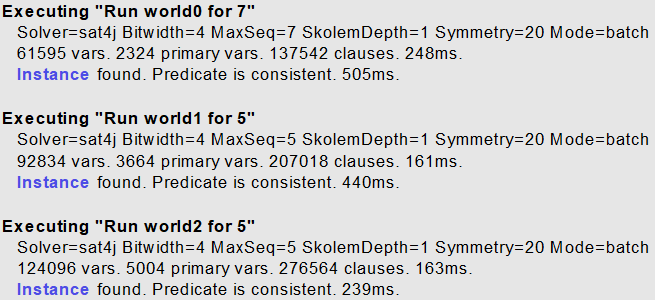
\includegraphics[width=\textwidth,height=\textheight,keepaspectratio]{./Images/Alloy/predicatesExecution.png}
           \vspace*{-0.5cm}
  \caption{Alloy Analysis Results}
\end{figure}



\def\fillandplacepagenumber{%
 \par\pagestyle{empty}%
\vbox to 0pt{\vss}\vfill
\vbox to 0pt{\baselineskip0pt
   \hbox to\linewidth{\hss}%
   \setlength{\footskip}{70pt}
   \baselineskip\footskip
   \hbox to\linewidth{%
     \hfil\thepage\hfil}\vss}}

\begin{landscape}
\begin{figure}[h]
\vspace*{-2cm}
\noindent
\centering
\centerline{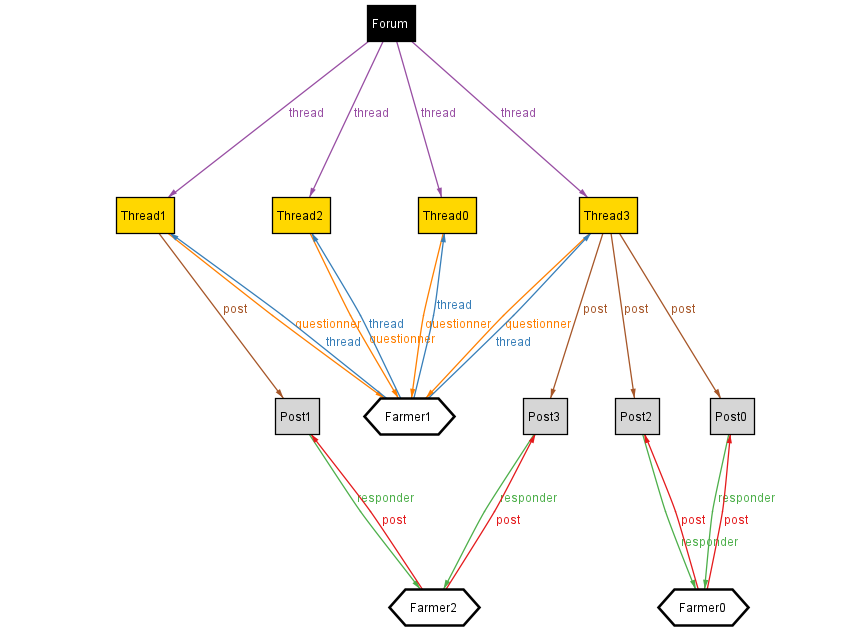
\includegraphics[scale = 0.6]{./Images/Alloy/DiscussionForum.png}}
    \caption{Generated World0 - Discussion Forum}
    \vspace*{-12cm}
\end{figure}
\fillandplacepagenumber
\end{landscape}


\newpage
\begin{landscape}
\begin{figure}[h]
\vspace*{-2cm}
\noindent
\centering
\centerline{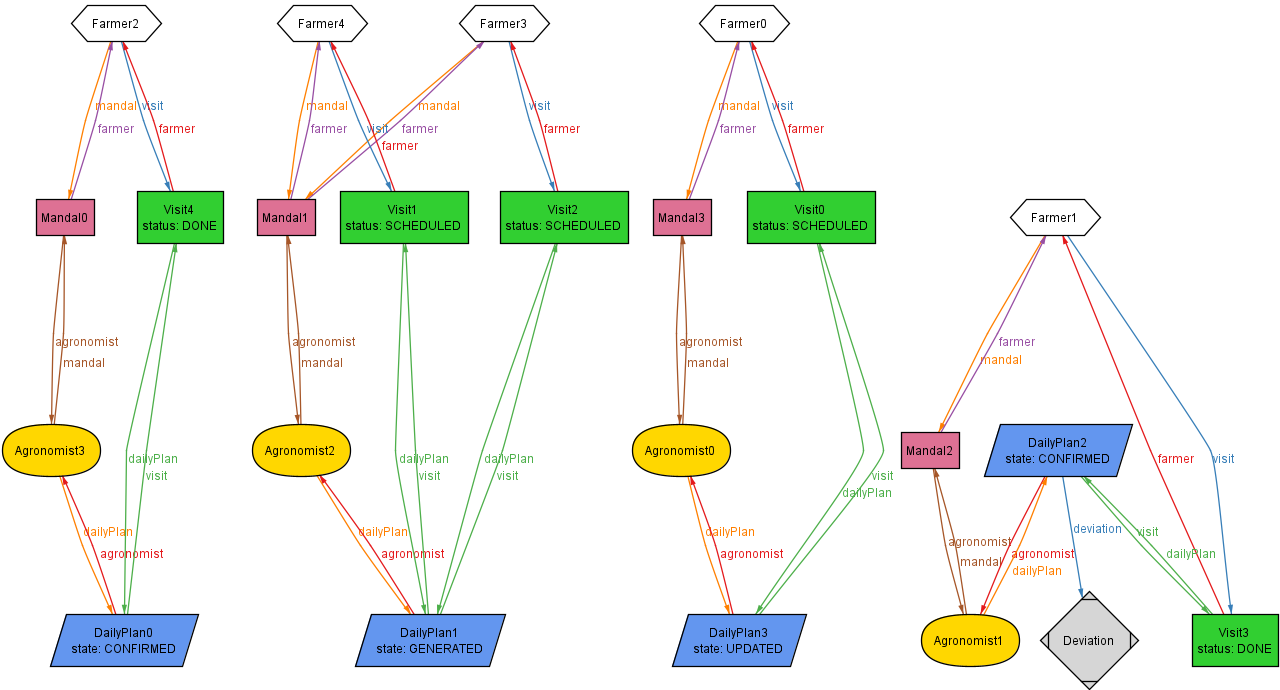
\includegraphics[scale= 0.6]{./Images/Alloy/DailyPlan.png}}
    \vspace*{-0.5cm}
  \caption{Generated World1 - Daily Plan}
    \vspace*{-12cm}
\end{figure}
    \fillandplacepagenumber
\end{landscape}

\newpage
\begin{landscape}
\begin{figure}[h]
\vspace*{1cm}
\noindent
\centering
\centerline{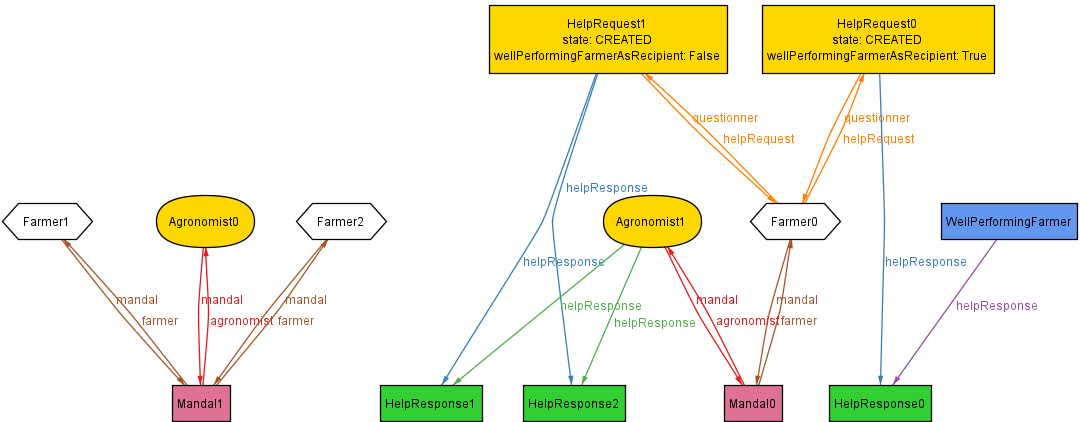
\includegraphics[scale= 0.6]{./Images/Alloy/HelpRequest.png}}
  \caption{Generated World2 - Help Request}
    \vspace*{-3cm}
\end{figure}
    \fillandplacepagenumber
\end{landscape}
